\documentclass{beamer}

\usetheme{Madrid}
\usepackage[utf8]{inputenc}
\usepackage[T1]{fontenc}
\usepackage{graphicx}
\usepackage{booktabs}
\usepackage{amsmath}

\graphicspath{{../static/}{../outputs/}}

\title[Road Segmentation]{Road Segmentation from Satellite Imagery}
\subtitle{A Comparison of Deep Learning and Traditional Baselines}
\author[Monteiro, Xavier]{William Wayn Monteiro \and Maysa Xavier}
\institute[UWS]{%
  COMP11069 -- Data Mining and Visualisation \\
  University of the West of Scotland%
}
\date{2025/2026}

% ---------------------
\begin{document}

\begin{frame}
  \titlepage
\end{frame}

\begin{frame}{Outline}
  \tableofcontents
\end{frame}

% =====================
\section{The Problem}

\begin{frame}{The Problem}
  \begin{columns}[T]
    \column{0.55\textwidth}
    \begin{block}{The intuition}
      Imagine holding a satellite photograph and being asked to draw every road.
      Your eye finds them immediately: thin grey threads snaking through fields.
      Your brain reads \textit{context}.
    \end{block}
    \vspace{0.5em}
    A computer sees only numbers.
    The grey of asphalt in full sun is nearly identical to dry riverbed in shadow.

    \vspace{0.5em}
    \textbf{The signal is spatial, not spectral.}

    \column{0.45\textwidth}
    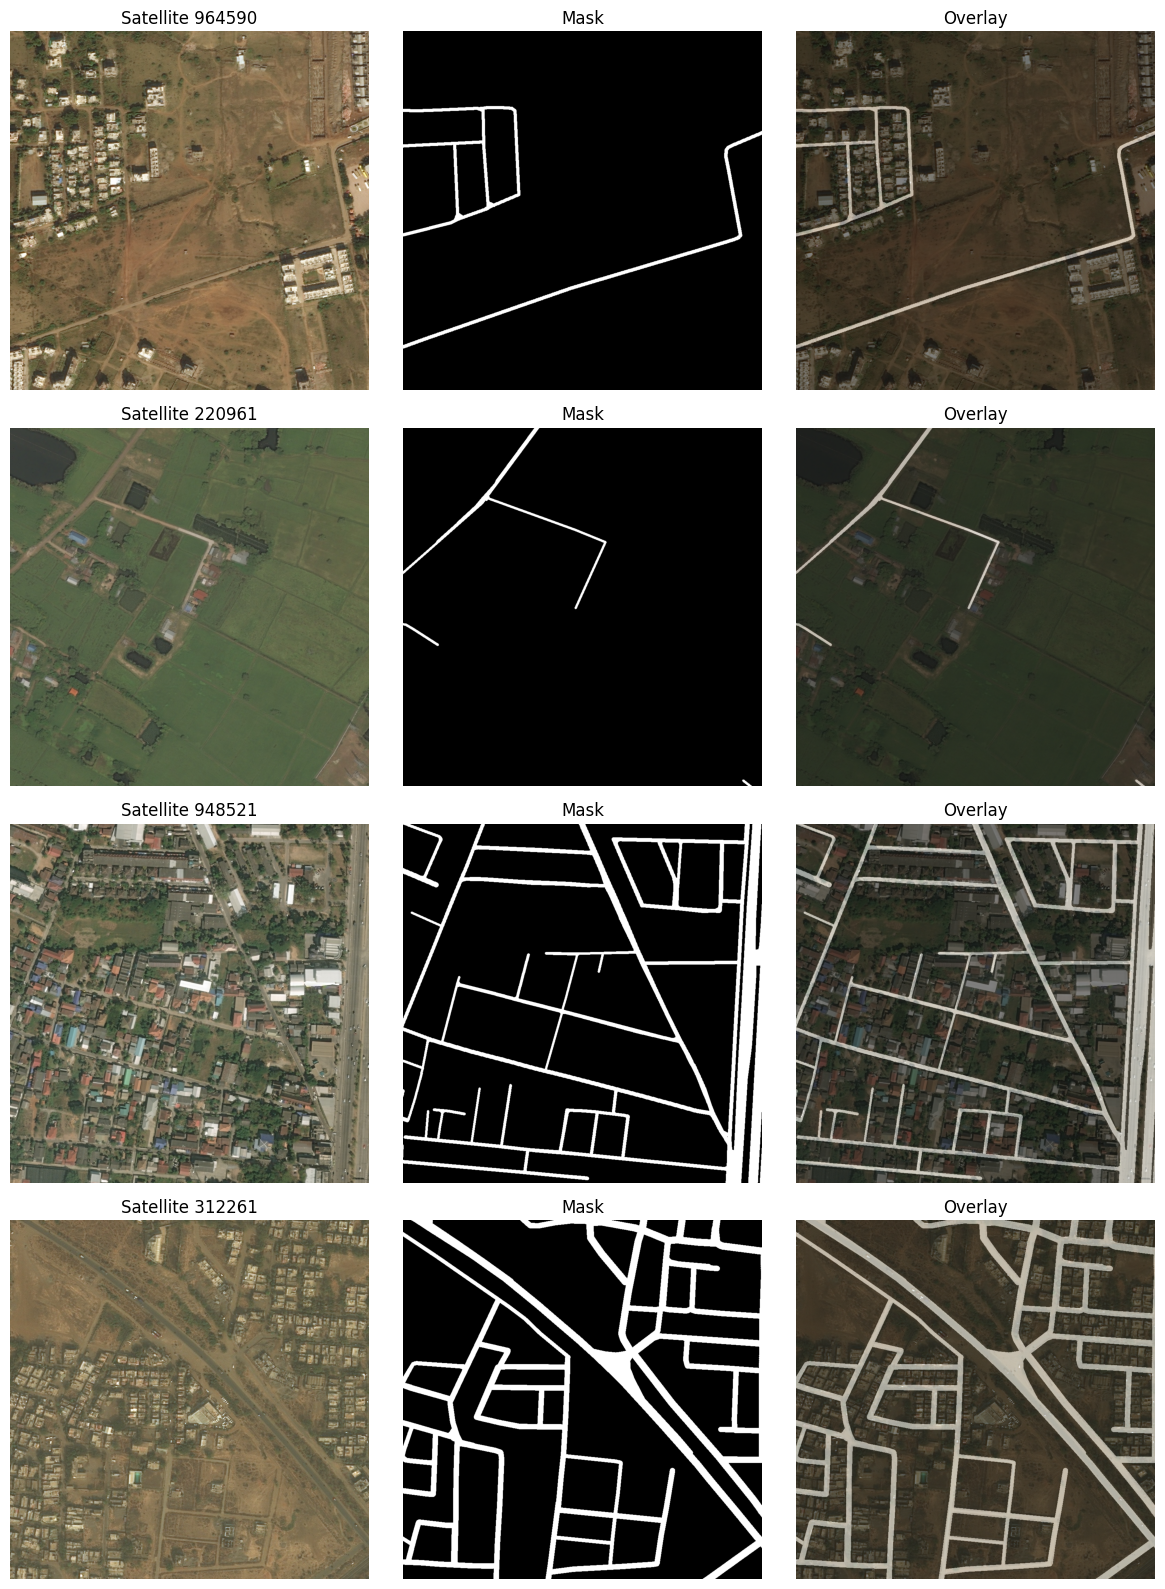
\includegraphics[width=\linewidth]{images_example.png}
  \end{columns}
\end{frame}

\begin{frame}{Two Challenges That Drive Everything}
  \begin{enumerate}
    \item \textbf{Class imbalance}
    \begin{itemize}
      \item Roads cover only 4--8\% of each tile
      \item Predicting ``no road'' everywhere $\Rightarrow$ $>$92\% pixel accuracy
      \item[$\Rightarrow$] We use \textbf{IoU}, not accuracy
    \end{itemize}
    \vspace{0.8em}
    \item \textbf{Thin, elongated structures}
    \begin{itemize}
      \item After resizing to $256\times256$, rural roads are 3--5 pixels wide
      \item A model that discards spatial resolution cannot recover them;
            the information is already gone
      \item[$\Rightarrow$] Architecture must \textit{preserve} spatial detail,
            not reconstruct it
    \end{itemize}
    \vspace{0.8em}
    \centering
    
\includegraphics[width=0.7\linewidth]{iou_diagram}
    \small\centering
    \textit{The metric that matters: IoU counts overlap vs.\ union}
  \end{enumerate}
  \vspace{0.5em}
  \centering
  \textit{These two observations will govern every choice we make.}
\end{frame}

% =====================
\section{Dataset \& EDA}

\begin{frame}{DeepGlobe Road Extraction}
  \begin{columns}[T]
    \column{0.55\textwidth}
    \begin{itemize}
      \item $1024\times1024$ px, 50\,cm/pixel GSD
      \item Thailand, Indonesia, India
      \item \textbf{803} train / \textbf{171} val / 172 test
      \item Resized to $256\times256$ for training \\
            (trade-off discussed in limitations)
    \end{itemize}
    \vspace{0.5em}
    The dataset spans wide urban arteries to thin dirt tracks --- a broad range of difficulty.

    \column{0.45\textwidth}
    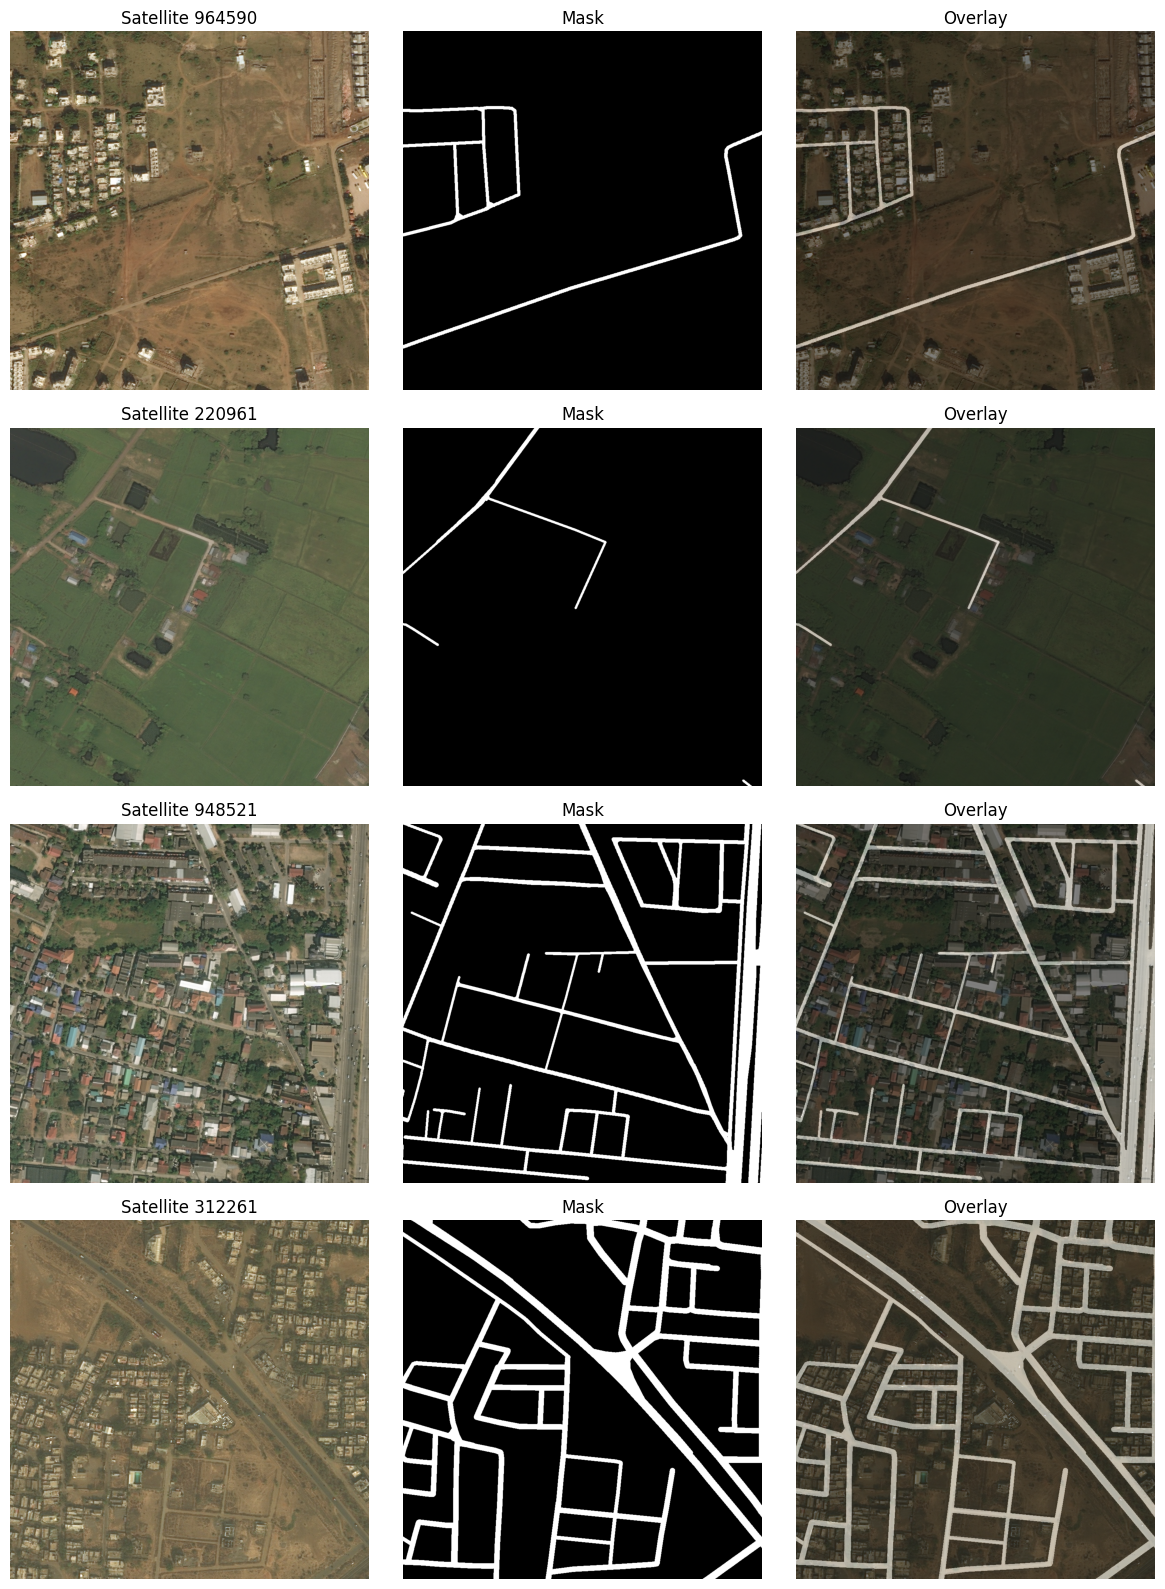
\includegraphics[width=\linewidth]{images_example.png}
  \end{columns}
\end{frame}

\begin{frame}{What the Data Tells Us --- Before Any Experiment}
  Three observations from the EDA that constrain every method we will try.
  \vspace{0.3em}
  \begin{block}{Spectral heterogeneity}
    Asphalt in sun: bright. Same road under canopy: dark. Dry earth track: nearly white.
    Any colour threshold faces an \textbf{impossible trade-off}.
  \end{block}
  \vspace{0.2em}
  \begin{block}{Thin structures}
    3--5 pixel-wide roads at $256\times256$.
    Architecture must \textbf{preserve}, not reconstruct, spatial resolution.
  \end{block}
  \vspace{0.2em}
  \begin{block}{Class imbalance}
    4--8\% road pixels per tile.
    Accuracy is meaningless; \textbf{IoU penalises both error types equally}.
  \end{block}
\end{frame}

% =====================
\section{Methods}

\begin{frame}{Our Approach: A Ladder of Complexity}
  \begin{center}
    \begin{tabular}{clll}
      \toprule
      Rung & Method & What it adds \\
      \midrule
      1 & RGB Thresholding       & Colour statistics \\
      2 & K-Means Clustering     & Colour grouping \\
      3 & \textbf{U-Net}         & Spatial context + local detail \\
      4 & DeepLabV3              & Global context + pretraining \\
      \bottomrule
    \end{tabular}
  \end{center}
  \vspace{0.8em}
  \centering
  We start simple. We add complexity only when the data demands it.
\end{frame}

\begin{frame}{Rungs 1 \& 2: Classical Baselines}
  \begin{columns}[T]
    \column{0.52\textwidth}
    \textbf{RGB Thresholding}
    \begin{itemize}
      \item KS test finds the best colour threshold from 50 training images
      \item 5 strategies swept; best selected by IoU
      \item Expected to fail --- EDA told us why before we ran it
    \end{itemize}
    \vspace{0.5em}
    \textbf{K-Means} ($k=2$)
    \begin{itemize}
      \item Algorithm finds colour clusters without supervision
      \item Clusters labelled road/non-road by overlap with masks
      \item Same fundamental limit: pixel-level, no spatial context
    \end{itemize}

    \column{0.48\textwidth}
    \includegraphics[width=\linewidth]{baselines/kmeans_results.png}
  \end{columns}
\end{frame}

\begin{frame}{Rung 3: U-Net}
  \begin{columns}[T]
    \column{0.55\textwidth}
    Proposed by Ronneberger, Fischer \& Brox (2015) for biomedical segmentation. \\[0.4em]
    The defining feature: \textbf{skip connections}. \\
    Feature maps from each encoder stage concatenate directly into the matching decoder. \\[0.4em]
    \begin{itemize}
      \item High-resolution detail is \textit{preserved}, not reconstructed
      \item Exactly what the thin-road observation demanded
      \item 31.0\,M parameters, trained from scratch
      \item 30 epochs, Adam $\eta=10^{-4}$, BCE loss
    \end{itemize}

    \column{0.45\textwidth}
    \includegraphics[width=\linewidth]{unet/training_curves.png}
    \vspace{0.2em}
    \small\centering
    Clean convergence: val.\ loss tracks training throughout.
  \end{columns}
\end{frame}

\begin{frame}{Rung 4: DeepLabV3}
  A different philosophy applied to the same problem. \\[0.4em]
  \textbf{Atrous (dilated) convolutions} expand the receptive field \textit{without} reducing spatial dimensions. \\[0.4em]
  \textbf{ASPP} combines multiple dilation rates to aggregate multi-scale context. \\[0.4em]
  \begin{itemize}
    \item ResNet-50 backbone, pretrained on ImageNet
    \item 39.6\,M parameters, fine-tuned end-to-end
    \item Designed for objects that appear at many scales
  \end{itemize}
  \vspace{0.5em}
  \begin{alertblock}{Our hypothesis, before training}
    U-Net preserves local detail. DeepLabV3 aggregates global context.
    Roads are thin, local structures.
    We will see whether that distinction makes a difference.
  \end{alertblock}
\end{frame}

% =====================
\section{Results}

\begin{frame}{Results: Quantitative}
  \begin{center}
    \begin{tabular}{lcc}
      \toprule
      Method                  & Val.\ IoU        & Parameters \\
      \midrule
      RGB Thresholding (KS)   & $\sim$0.15--0.25 & -- \\
      K-Means ($k=2$)         & $\sim$0.20--0.30 & -- \\
      DeepLabV3 (ResNet-50)   & 0.348            & 39.6\,M \\
      U-Net ($512\times512$)  & 0.565            & 31.0\,M \\
      \textbf{U-Net ($256\times256$)} & \textbf{0.588}   & 31.0\,M \\
      \bottomrule
    \end{tabular}
  \end{center}
  \vspace{0.5em}
  We can notice that the gap is not marginal: U-Net leads DeepLabV3 by \textbf{0.24 IoU points}
  and outperforms both baselines by over \textbf{0.30 points}. \\[0.4em]
  The ladder produces a clear ordering --- with one surprise: DeepLabV3 falls \textit{below}
  what its size and pretraining would suggest.
\end{frame}

\begin{frame}{Results: Visual Comparison}
  \begin{columns}[T]
    \column{0.5\textwidth}
    \centering
    \textbf{U-Net}
    \includegraphics[width=\linewidth]{unet/unet_prediction_3_valid.png}
    \small Sharp, connected outlines; thin rural tracks recovered.

    \column{0.5\textwidth}
    \centering
    \textbf{DeepLabV3}
    \includegraphics[width=\linewidth]{deeplabv3/deeplabv3_prediction_3_valid.png}
    \small Road \textit{regions} found, but edges blurred and thin segments dropped.
  \end{columns}
  \vspace{0.4em}
  \centering
  We can notice that this is precisely the failure mode one would predict for a model
  that favours global context over fine spatial precision.
\end{frame}

% =====================
\section{Discussion}

\begin{frame}{The Resolution Paradox: $256\times256$ vs $512\times512$}
  We experimented with higher resolution ($512\times512$) to better preserve thin roads.
  \vspace{0.5em}
  
  \begin{block}{The Paradox}
    \begin{itemize}
      \item \textbf{$256\times256$ (IoU 0.588):} Downsampling heavily blurs thin roads, artificially thickening them. The model overlaps these inflated areas more easily, resulting in higher mathematical IoU.
      \item \textbf{$512\times512$ (IoU 0.565):} Higher resolution keeps roads thinner and more accurate to reality. However, IoU heavily penalises slight 1-pixel misalignments at the boundaries.
    \end{itemize}
  \end{block}
  \vspace{0.5em}
  \textbf{Takeaway:} The higher resolution model preserves the true topology of the road network better qualitatively, even if strict exact-pixel IoU matching decreases.
\end{frame}

\begin{frame}{Why U-Net Outperforms DeepLabV3}
  I think this result deserves a careful interpretation rather than a quick dismissal. \\[0.4em]
  DeepLabV3 is, by standard measures, the stronger model: more parameters, ImageNet
  pretraining, and a multi-scale context module built for recognising objects at many scales. \\[0.4em]
  \begin{block}{I believe the explanation is a design mismatch}
    ASPP aggregates multi-scale context --- helpful when the same object appears at
    many sizes (a car far away versus a car up close). \\[0.3em]
    Roads at $256\times256$ are not that kind of object.
    What matters is not ``what is happening across the whole image'' but
    ``what is happening in the 5 pixels around me.'' \\[0.3em]
    U-Net's skip connections answer that local question directly.
    ASPP's global pooling does not.
  \end{block}
\end{frame}

\begin{frame}{Paths Forward \& Limitations}
  \begin{columns}[T]
    \column{0.55\textwidth}
    \textbf{What could push further:}
    \begin{itemize}
      \item BCE + Dice loss --- directly optimises an IoU proxy; known to help under class imbalance
      \item Boundary-aware loss --- to compensate for the strictness of IoU on high-resolution ($512\times512$) fine structures
      \item Test-time augmentation --- typically +1--3 IoU points at no training cost
    \end{itemize}

    \column{0.45\textwidth}
    \textbf{Honest limitations:}
    \begin{itemize}
      \item One geographic region only (South \& SE Asia)
      \item No evidence of generalisation to other sensors or seasons
      \item Test labels withheld by the challenge
    \end{itemize}
  \end{columns}
\end{frame}

% =====================
\section{Conclusion}

\begin{frame}{The Main Lesson}
  \begin{center}
    \large
    A careful reading of the data is more valuable than\\
    a reflexive choice of the most powerful model.
  \end{center}
  \vspace{0.8em}
  \begin{itemize}
    \item Understanding that roads are \textbf{thin}, \textbf{sparse}, and \textbf{spectrally
          heterogeneous} pointed us to U-Net's design before we trained a single epoch
    \item The results confirmed that intuition: \\
          \textbf{U-Net 0.588} vs.\ DeepLabV3 0.348 and classical baselines $\leq$ 0.30
    \item Inductive bias matters more than model size when the task has a clear structural
          requirement
  \end{itemize}
  \vspace{0.5em}
  \centering
  \textit{Thank you.}
\end{frame}

\end{document}
